\documentclass[a4paper,12pt]{report}
\usepackage[fiche,niveau={1MA1},nfiche={21}, annee={Emilie-Gourd, 2024--2025},
auteur={ns},theme={Géométrie -- Preuves à connaître}]{packages/bandeaux}
\usepackage{packages/boites}
\usepackage{packages/courslatex}
\usepackage{packages/fontes}
\usepackage{packages/mathenv}
\allowdisplaybreaks

\begin{document}
\begin{thm}
	Deux angles opposés par le sommets sont isométriques.
\end{thm}
\begin{proof}
	Soient deux angles $\alpha$ et $\beta$ opposés par le sommet. On trace l'angle $\gamma$ comme dans le schéma ci-dessous. On a 
	\[\beta+\gamma=180^\circ\]
	et 
	\[\alpha+\gamma=180^\circ.\]
	Ainsi, 
	\[\alpha=\beta=180^\circ-\gamma.\]
\begin{center}
	\begin{tikzpicture}
		  % Définition des points
  \tkzDefPoint(0,0){O}
  \tkzDefPoint(4,0){A}
  \tkzDefPoint(-4,0){C}
  \tkzDefPoint(3,2){B}
  \tkzDefPoint(-3,-2){D}
  % Tracé des droites
  \tkzDrawSegment(A,C)
  \tkzDrawSegment(B,D)
  % Marquage d'un des angles opposés par le sommet
  \tkzMarkAngle[size=0.8cm, mark=none, dashed](B,O,C)
  \tkzLabelAngle[pos=1.2](B,O,C){$\gamma$}
  \tkzMarkAngle[size=0.8cm, mark=none](C,O,D)
  \tkzLabelAngle[pos=1.2](C,O,D){$\beta$}
  \tkzMarkAngle[size=0.8cm, mark=none](A,O,B)
  \tkzLabelAngle[pos=1.2](A,O,B){$\alpha$}
	\end{tikzpicture}
\end{center}
\end{proof}
\begin{thm}
	Soient deux droites $d$ et $d'$ et $\alpha$ et $\beta$ deux angles alternes-internes définis sur ces deux droites par une troisième droite sécante quelconque. Alors on a : $d||d '\iff \alpha = \beta$.
\end{thm}
\begin{proof}
La situation est la suivante où on note la troisième droite $d''$. 

\begin{center}
\begin{tikzpicture}[scale=1]
  % Première droite (AB) : y = 0,5\,x
  \tkzDefPoint(0,0){A}
  \tkzDefPoint(5,2.5){B}
  % Seconde droite (CD) parallèle à AB : y = 3+0,5\,x
  \tkzDefPoint(0,2.5){C}
  \tkzDefPoint(5,5.5){D}
  % Transversale coupant AB en E et CD en F
  \tkzDefPoint(2,1){E} % E appartient à AB (car 1 = 0,5×2)
\tkzDefMidPoint(C,D) \tkzGetPoint{F}
  % Tracé des segments
  \tkzDrawLine(A,B)
\tkzLabelLine[pos=1.25,right](A,B){$(d)$}
  \tkzDrawLine(C,D)
\tkzLabelLine[pos=1.25,right](C,D){$(d')$}
\tkzDrawLine[add = 0.5 and 0.5](E,F)
\tkzLabelLine[pos=1.25,above right](E,F){$(d'')$}
  % Marquage des angles alternes internes
  \tkzMarkAngle[size=0.7cm, mark=none](B,E,F)
  \tkzLabelAngle[pos=1.2](B,E,F){$\alpha$}
  \tkzMarkAngle[size=0.7cm, mark=none](C,F,E)
  \tkzLabelAngle[pos=1.2](C,F,E){$\beta$}
  \tkzDefPointBy[homothety = center F ratio 1.5](E)\tkzGetPoint{G}
  \tkzMarkAngle[size=0.7cm, mark=none, dashed](A,E,G)
  \tkzLabelAngle[pos=1.2](A,E,G){$\gamma$}
\end{tikzpicture}
\end{center}

Remarquons que $\alpha$ et $\gamma$ sont opposés par le sommet, donc isométriques. De plus, $\gamma$ et $\beta$ sont correspondants. Par l'axiome des angles correspondants, $\gamma=\beta \iff d||d'$, donc $\alpha=\beta \iff d|| d'$. 


\end{proof}
\newpage

\begin{thm}
	La somme des angles dans un triangle vaut $180^\circ$.
\end{thm}
\begin{proof}
	Soit un triangle $ABC$. On trace la droite parallèle à $AB$ passant par le point $C$. On place deux points $D$ et $E$ sur la droite de part et d'autre de $C$ (c.f. le croquis ci-dessous).

	\begin{center}
	\begin{tikzpicture}
\tkzDefPoints{0/0/A,5/0/B,4/3/C,1/3/D,6/3/E}
\tkzDrawPolygon(A,B,C)
\tkzDrawLine[dashed](E,D)
\tkzDrawPoints(A,B,C,D,E)
\tkzLabelPoints(A,B)
\tkzLabelPoints[above](C,D,E)
\end{tikzpicture}	
	\end{center}

On a que $\widehat{ACD}$ et $\widehat{CAB}$ sont alternes-internes et $\widehat{ECB}$ et $\widehat{ABC}$ sont alternes-internes.  

Puisque les droites $DE$ et $AB$ sont parallèles (par construction), par le théorème des angles alternes-internes, \begin{equation}\label{eq:1}\widehat{ACD}=\widehat{CAB}\end{equation} et \begin{equation}\label{eq:2}\widehat{ECB}=\widehat{ABC}\end{equation}

De plus, $D,C,E$ sont alignés, donc
\[\widehat{ACD}+\widehat{ACB}+\widehat{ECB}=180^\circ\]
et par \eqref{eq:1} et \eqref{eq:2},
\[\widehat{CAB}+\widehat{ACB}+\widehat{ABC}=180^\circ\]
\end{proof}

\end{document}
